%
%   Chapter Related Works
%
%   Qing-Cheng Li (r01922024 at csie dot ntu dot edu dot tw)
%   R.O.C.103.07
%
\chapter{相關研究與文獻}
\label{c:related}

% FIXME - 需要潤飾。
本章將介紹相關的研究:知識庫加速(Knowledge Base Acceleration)方面相關的研究,
及相關的資源:結構化的知識庫(Structural Knowledge Bases)與實體間的關係(Relations between Entities)。

%
%   KBA
%
\section{知識庫加速}
% KBA Overall View
% BIT
% H*****

\cite{kba2012}
\cite{kba2013}

\cite{kba-hltoce}
\cite{kba-msra}

\cite{kba-entity-detection}

%
%   Structural KB
%
\section{結構化的知識庫}
% TODO

\cite{freebase}
\cite{dbpedia}
\cite{yago}

%YAGO

%
%   Pattern and Relation
%
\section{實體間的關係}

知識隨著時間變化是可能產生改變的,
\cite{relationsByTime} 提到有些實體間的關係是相對恆常的,例如《1Q84》的作者是村上春樹;
而有些關係則是隨著時間而變動的,例如美國的總統是布希,只有在某一段時間內是正確關係。
此研究將實體間的關係分為是否為恆常(Constant)或是否唯一(Unique),
人工挑選1,000組關係並利用時間、實體出現在特定時段內的頻率、文法等特徵對關係進行分類。

\cite{reverb} 建立了一套開放資訊擷取系統(Open Information Extraction System),
透過動詞表示的詞彙與句法限制,以<arg1, relation, arg2>的形式自動擷取出實體間的關係,
不限於人工標定的關係。

\cite{wisenet} 則利用Wikipedia文具中的連結作為特徵擷取條目間的關係,
由於同一種關係可能由不同的語句樣式(Patterns)來表達,
此研究應用了Wikipedia條目分類資訊來分類同義樣式。

\cite{patty2012}及\cite{patty}建立了一個名為PATTY的分類集(Taxonomy),
將用來表達關係的樣式進行分類,將同義樣式合併,並附上實體類別資訊,
將關係表達為「<type 1> \emph{Pattern} <type 2>」,Type 1和Type 2是實體的類別,
而Pattern則由單字(Words)、詞性標記(Part-Of-Speech Tags)、萬用字元(Wildcards)所組成,
例如「<person>'s [adj] voice * <song>」。   % FIXME - Example

PATTY自Wikipedia、New York Times抽取句子,以史丹佛剖析器(Stanford Parser\footnote{http://nlp.stanford.edu/software/lex-parser.shtml})對句子建立剖析樹,
以YAGO作為實體的字典,判斷若句子中有兩個實體,則把兩實體間在樹上的最短路徑上的字句擷取出來作為樣式,並進一步合併樣式為同義樣式集(Pattern Synset)。

對每一個樣式,都存在一組支持集(Support Set),由符合樣式的實體對(Pairs of entites)所組成。
透過支持集的大小,對每個樣式計算計算了一個信心值(),將樣式中的實體類別從類別改為類別繼承架構中的父節點,


%PATTY, WiSeNet

%\begin{figure}
%\centering
%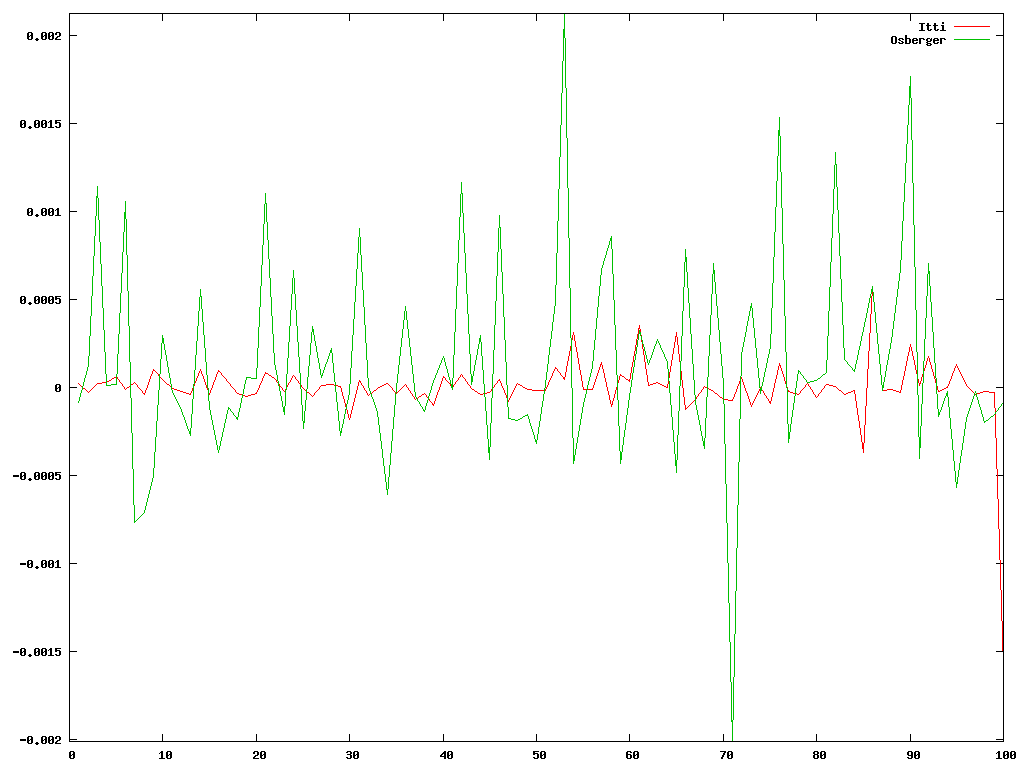
\includegraphics[width=0.45\textwidth]{images/kl}
%\caption{kl-distance}
%\label{kl}
%\end{figure}

%\begin{table}[t]
%\begin{center}
%\begin{tabular}{lcc}
%
%\hline
%                    &  {\small Itti's method}     & {\small Fuzzy growing}    \\
%\hline
%{\small Precision}           &  0.4475    & 0.4506 \\
%{\small Recall}              &  0.5515    & 0.5542 \\
%\hline
%
%\end{tabular}
%\caption[Evaluation of FOA sets]{\small Evaluation of FOA sets. } \label{t:FOA}
%\end{center}
%\end{table}

